\documentclass[conference]{IEEEtran}
%\IEEEoverridecommandlockouts
% The preceding line is only needed to identify funding in the first footnote. If that is unneeded, please comment it out.
\usepackage{cite}
\usepackage{amsmath,amssymb,amsfonts}
\usepackage{algorithmic}
\usepackage{graphicx}
\usepackage{textcomp}
\usepackage{xcolor}
\usepackage{tabularx}
\usepackage{multirow}
\usepackage{subcaption}
\usepackage{float}
\usepackage{dblfloatfix}
\usepackage{placeins}
\usepackage[hidelinks]{hyperref}




\def\BibTeX{{\rm B\kern-.05em{\sc i\kern-.025em b}\kern-.08em
    T\kern-.1667em\lower.7ex\hbox{E}\kern-.125emX}}
\begin{document}

\title{Time-optimal Flying a VTOL Drone}

\author{\IEEEauthorblockN{Larissa Rickler}
\IEEEauthorblockA{(03697651)\\
larissa.rickler@tum.de}
\and
\IEEEauthorblockN{Leonardo Igler}
\IEEEauthorblockA{(03702035)\\
leonardo.igler@tum.de}






}

\maketitle




\begin{abstract}

This milestone report describes our group's first experiments in training a drone to follow simple 2D trajectories using deep reinforcement learning methods.

\end{abstract}

%\begin{IEEEkeywords}
%reinforcement learning, VTOL drone, neural network controller
%\end{IEEEkeywords}

\section{Methods}
\label{sec:methods}
We used an actor-critic algorithm as approximator. The applied optimization algorithm is Adam.
The actor network produces actions learned via the Proximal Policy Optimization (PPO). Both actor and critic are multilayer perceptrons (MLP), see Table \ref{table:network} and Figure \ref{fig:actor} for details on their architectures.
\begin{table*}[t]
\centering
\caption{Network architecture.}
\begin{tabular}{c|c|c|c|c|c|c|c} 
 \hline 
 Network & Type & Input & Hidden Layer & Activation & Last Layer & Output & Output Size \\ [0.1ex] 
 \hline
 \hline
 \multirow{2}*{actor} & \multirow{2}*{MLP} & \multirow{2}*{observation} & \multirow{2}*{2x128} & \multirow{2}*{tanh} & 1x128 & action mean & 2 \\ [0.1ex]
    & & & & & 1x128 & action variance & 2 \\ [0.1ex]
 \hline
 critic & MLP & observation & 2x128 & tanh & 1x128 & value & 1 \\ [0.1ex] 
 \hline
\end{tabular}
\label{table:network}
\end{table*}

The chosen observation space and reward function are based on the suggestions of Penicka et al. \cite{Penicka_2022}.
The observations consist of two parts: the VTOL drone's state (world position, body orientation, as well as the translational and rotational velocities) and the relative path to the next two waypoints. 
The VTOL drone model provided by Flyonic \cite{flyonic} allows four possible actions: 
regulating thrusts of two propellers and adjusting angles of two flaps. 
% setting the rotation speed of the two propellers individually, as well as adjusting the angle of the two flaps the drone possesses.
In Figure \ref{fig:actor} both observation and action space are illustrated.
\begin{figure}[ht]
    \centering
    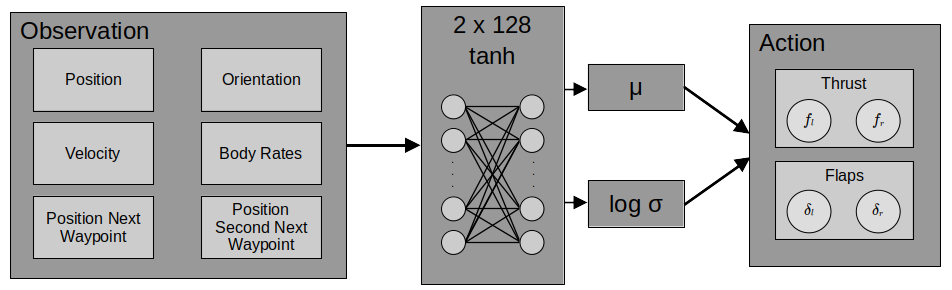
\includegraphics[width=8cm]{images/actor_short.png}
    \caption{Illustration of the actor network with the used observation and action space.}
    \label{fig:actor}
\end{figure}

The reward function consist of five parts: encouraging progression along the trajectory (connected lines between $n$ waypoints $g_1,...,g_n$) in every time step, rewarding the overall reached distance along the trajectory, rewarding reached waypoints, penalizing high body rates $\omega$ and penalizing inactivity. To calculate the progress at position $p$ we define the closest point on the trajectory as $\psi(p)$ and its corresponding line segment index as $l(p)$. See an example illustration in Figure \ref{fig:trajectory}.
\begin{figure}[b]
    \centering
    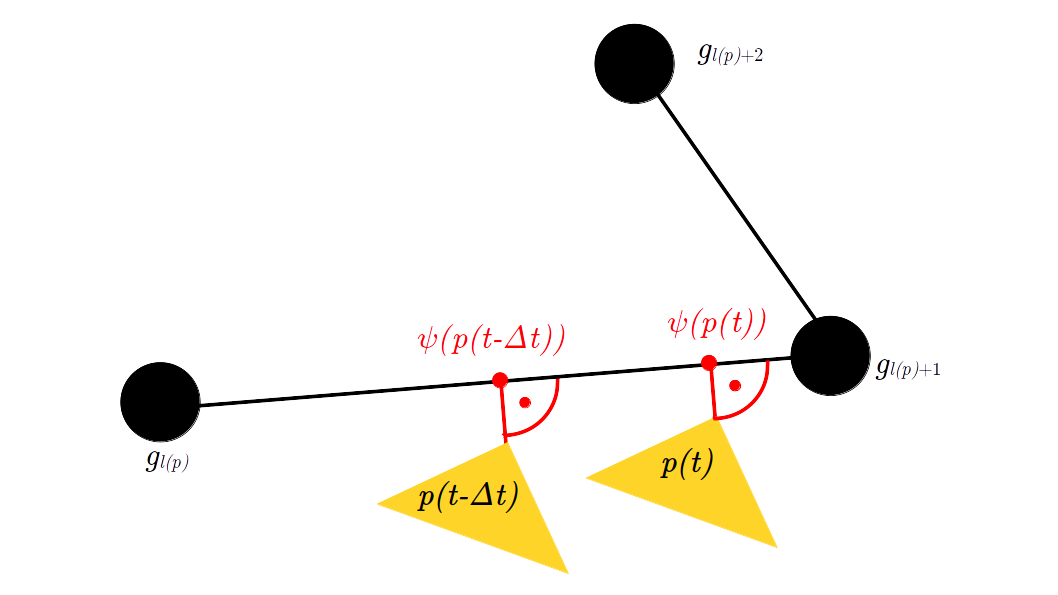
\includegraphics[width=6.5cm]{images/trajectory.png}
    \caption{Illustration of trajectory with three waypoints. The nearest point $\psi(p)$ on trajectory from drone at position $p$ and its corresponding line segment index $l(p)$ is used to calculate the progress in each time step $\Delta t$ and the reached distance.}
    \label{fig:trajectory}
\end{figure}
The total reward function $r(t)$ at time $t$ is defined as 
\begin{align*}
r(t) = k_p r_p(t) + k_s s(p(t)) + k_{wp} r_{wp} + k_\omega \|\omega\| - fall,
\end{align*}
with the reached distance along the trajectory $s(p(t))$ and the progress reward at each time step $r_p(t)$ being defined as
\begin{align*}
    &s(p) = \sum_{i=1}^{l(p) - 1} \| g_{i+1} - g_i \| + \|\psi(p) - g_{l(p)}\|, \\
    &r_p(t) = s(p(t))-s(p(t- \Delta t)).
\end{align*}
The reached distance $s(p(t))$ is part of the reward function to counteract possible singularities due to sharp corners of the trajectory and the minimum distance projection. The reward $r_{wp}$ was payed, if the drone reached a waypoint within a distance $d_{wp}$ smaller than a tolerance $r_{tol}$ for the first time. The penalty term $fall$ was only subtracted if the drone fell under $-1$m due to inactivity. The contribution of each reward part is scaled by the hyperparameters $k_p$, $k_s$, $k_{wp}$ and $k_{\omega}$.

We initially focused on learning a slow and stable flying policy, henceforth referred to as \textit{slow learning phase}. Therefore, the hyperparameters $k_s$ and $k_p$ were scaled by a factor $s_m$ that encouraged translation velocities between $v_{min}$ and $v_{max}$. This factor also motivates the drone to stay within a distance of $d_{max}$ to the trajectory. The scaling factor $s_m$ is calculated as
\begin{align*}
 & s_m = s_{v} \cdot s_{gd}, \\
 & s_{v} = \min(1, 10^{v_{max}-||v||}) \cdot \min(1, 10^{||v||-v_{min}}), \\
 & s_{gd} = \min(1,e^{ - \|p - \psi(p) \| + d_{max}}).
\end{align*}
For our training process the values in Table \ref{table:parameters} were used.
\begin{table}[h]
\centering
\caption{Parameters of the algorithm.}
\begin{tabular}{c c|c c} 
 \hline 
 Variable & Value & Variable & Value \\ [0.1ex] 
 \hline
 \hline
 $v_{min}$ [m/s] & $1.0$ & $v_{max}$ [m/s] & $3.0 $ \\ [0.2ex]
 $\Delta t$ [s] & $0.025$ & $fall$ [-] & 1 \\ [0.2ex]
 $n$ & 4 & $k_{wp}$ [-] & $10.0 n$ \\ [0.2ex]
 $r_{tol}$ [m] & 0.5& $r_{wp}$ & $\exp(d_{wp}/r_{tol})$ \\ [0.2ex]
 $k_p$ [-] & $5.0$ & $k_\omega$ [-] & 0.01 \\ [0.2ex] 
 $k_s$ [-] & $\frac{2v_{max}\Delta t}{\sum_{i=1}^{n-1} \|g_{i+1} -g_i\|}$ & $d_{max}$ [m] & 0.2 \\[2ex] 
 \hline
\end{tabular}
\label{table:parameters}
\end{table}

\section{Experiments}
\label{sec:experiments}
\begin{figure*}[t]
\centering
\begin{subfigure}[htb!]{0.3\textwidth}
    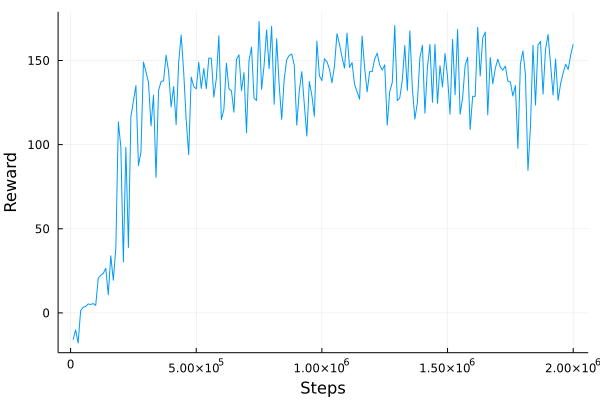
\includegraphics[width=\textwidth]{images/Reward_slow.png}
    \caption{Reward per step for the slow learning phase in 2D.}
    \label{fig:reward_slow}
\end{subfigure}
\hfill
\begin{subfigure}[htb!]{0.3\textwidth}
    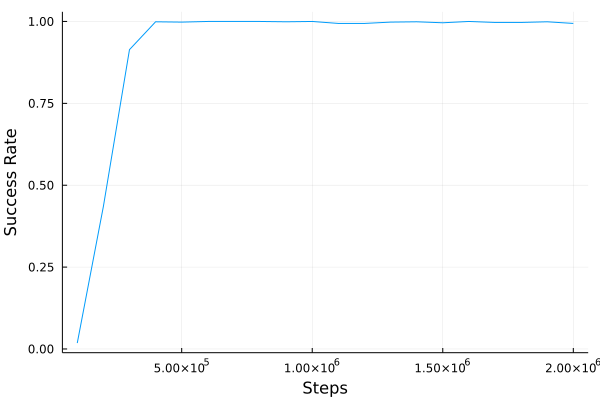
\includegraphics[width=\textwidth]{images/Success_slow.png}
    \caption{Success rate per step for the slow learning phase in 2D.}
    \label{fig:success_slow}
\end{subfigure}
\hfill
\begin{subfigure}[htb!]{0.3\textwidth}
    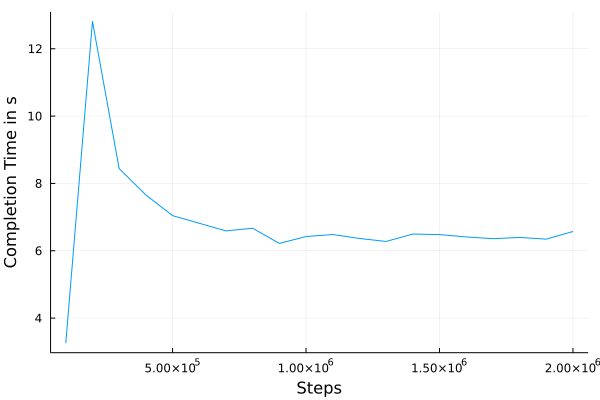
\includegraphics[width=\textwidth]{images/Time_slow.png}
    \caption{Completion time of successful attempts per step for the slow learning phase in 2D.}
    \label{fig:time_slow}
\end{subfigure}
\caption{Experimental setup described in Section \ref{sec:experiments}. Note that in \ref{fig:time_slow} the completion time in step 1 is set to zero, since there were no successful flights.}
\label{fig:results}
\end{figure*}
All the experiments were executed inside the Flyonic's physic simulation environment \cite{flyonic}. 
For the scope of our group's milestone report, we reduced our experiments to a 2D plane (xz-plane). We have disabled all forces that would conflict with this 2D-world, as well as the possible actions regarding the flaps of the drone. It is noteworthy that the gravity is still enabled, having an orientation antiparallel to the z-axis.
\par
The drone is trained for a total of two million time steps with a step size of $\Delta t$. 
In each episode a trajectory with 4 waypoints (including the starting point in the origin) is generated as follows:
The derivation from the previous point is randomly sampled from the uniform distributions $\mathcal{U}(-7, +7)$ for the x-axis and $\mathcal{U}(+1.5, +7)$ for the z-axis. Then, the guiding trajectory is given by the three straight lines connecting the waypoints. 
\par
A flight is considered a success, if each of the four points is passed within a tolerance of $r_{tol}$. This is also reflected through the chosen termination criteria. An episode terminates once one of the following conditions is met:
\begin{itemize}
    \item Drone falls 5 meters below the initial level
    \item Episode takes longer than $10.0 \cdot n$ seconds
    \item Drone deviates more than 5 meter from trajectory
    \item All waypoints were reached
\end{itemize}
\par
During training, every 100,000 steps the current state of the model is saved for further evaluation, which is topic of Section \ref{results}.

\section{Results}
\begin{figure*}[t]
    \centering
    \begin{subfigure}[htb!]{0.22\textwidth}
        \includesvg[width=\textwidth]{images/results/success_rate.svg}
        \caption{Success rate per step for both learning phases in 2D.}
        \label{fig:2D_success_rate}
    \end{subfigure}
    \hfill  
    \begin{subfigure}[htb!]{0.22\textwidth}
        \includesvg[width=\textwidth]{images/results/avg_velocity.svg}
        \caption{Average velocity per step for both learning phases in 2D.}
        \label{fig:2D_velocity}
    \end{subfigure}
    \hfill
    \begin{subfigure}[htb!]{0.22\textwidth}
        \includesvg[width=\textwidth]{images/results3D/success_rate_3D.svg}
        \caption{Success rate per step for both learning phases in 3D.}
        \label{fig:3D_success_rate}
    \end{subfigure}
    \hfill  
    \begin{subfigure}[htb!]{0.22\textwidth}
        \includesvg[width=\textwidth]{images/results3D/avg_velocity_3D.svg}
        \caption{Average velocity per step for both learning phases in 3D.}
        \label{fig:3D_velocity}
    \end{subfigure}
    
    \caption{Evaluation of our policy per training step. Discussed in Section \ref{sec:results}.}
    \label{fig:results}
\end{figure*}

To validate the trained policy, we tested it on 200 trajectories that were generated similarly as the training paths. We investigated the achieved success rate on reaching every point within the tolerance and the average velocity of the successful flights per training step for both the slow and fast learning phase. The fast flight policy was retrained with the model parameters after $0.5 \times 10^6$ of slow phase training. In \cite{videos} videos of the results of each of the following experiments can be found.

\subsection{Evaluation of 2D World Setting}
The success rate in the slow learning phase increases in a fast pace. After 500,000 steps the rate already consistently reaches values over 90\%, as seen in Figure \ref{fig:2D_success_rate}. The average velocity of a successful slow flight approached $3\frac{\text{m}}{\text{s}}$ which corresponds to $v_{max}$, see Figure \ref{fig:2D_velocity}.

Figure \ref{fig:2D_success_rate} also shows that the success rate in the fast learning phase remains in almost ever step by over 90\%, as . After $1.5 \times 10^6$ steps of the fast learning phase, the simulated elektra VTOL3 drone reaches speeds of up to $6\frac{\text{m}}{\text{s}}$ which is optimal for this model as illustrated in Figure \ref{fig:2D_velocity}.

\subsection{Evaluation of 3D World Setting}
In the slow learning phase, the quadrotor model's success rate consistently reaches values between 96\% and 100\% after $15.0 \times 10^6$ steps as shown in Figure \ref{fig:3D_success_rate}. This is probably due to its high agility. Figure \ref{fig:3D_velocity} shows that the average velocity again approaches $3\frac{\text{m}}{\text{s}}$ as encouraged by $v_{max}$. 

The high success rate remains over 96\% in the fast learning phase as illustrated in Figure \ref{fig:3D_success_rate}. After $40.0 \times 10^6$ steps the quadrotor's average speed seems to converge to $4\frac{\text{m}}{\text{s}}$ which was the value we chose for $v_{min}$ as illustrated in Figure \ref{fig:3D_velocity}. This is not time optimal yet. We hypothesize that the curriculum learning strategy needs to be extended to more phases in which $v_{min}$ is slowly increased to achieve even better results. 

\subsection{Evaluation on the Office Trajectory}
To compare our results to those of \cite{Penicka_2022}, we retrained our fast flight model on horizontal trajectories for another $40.0 \times 10^6$ steps. The trajectories were generated as in \eqref{equ:trajectory_generation} with $z_i \sim \mathcal{U}_3([-8.0,0.0] \times [-4.0,4.0] \times 0)$. We than generated a collision free trajectory to mimic the path optimal trajectories through the so called office environment. The office is one of the test environments used in \cite{Penicka_2022}. In \cite{office_environment} the environment and the generated trajectory is shown. Here we evaluated 30 runs. The success rate was 100\% even though the test trajectory had much sharper curves than the training trajectories. The average velocity during those runs were $7 \frac{\text{m}}{\text{s}}$. In Table \ref{table:compare} our results are compared with those of Penicka et al. The better results of their algorithm are due to an additional use of a path planning algorithm as well as their use of an low-level PID controller to convert their action signals to speed commands. This action modality has been identified as optimal for learned control policies for quadrotor by \cite{Controller_benchmarking}. 

\begin{table}[t]
\centering
\caption{Comparison of success rate, average completion time and best completion time in the office environment.}
                \begin{tabular}{c|c|c|c} 
                 \hline 
                  & success[\%] & avg. compl. time [s] & best. compl. time [s] \\ [0.1ex]
                  \hline
                  \hline
                 \cite{Penicka_2022} & 100 & 1.74 & 1.72 \\ [0.1ex] 
                 ours & 100 & 3.61 & 3.55 \\ [0.1ex] 
                 \hline
                 \end{tabular}
\label{table:compare}
\end{table}

\section{Future Work}
As stated in the previous section, the drone performs well for the models trained with the scaled reward functions. However, in order to achieve the desired time optimality, an unscaled reward should be applied. Regarding the performance of time optimal training strategy, further investigations need to be conducted. 
\par
Once the 2D case is optimized, the achieved progress will be generalized to the case of 3D trajectories. By then, the drone's whole set of action (propellers and flaps) will be unlocked, aiming to achieve time optimality using the full potential of the drone.






\bibliographystyle{IEEEtran}
\bibliography{milestone-report}

\end{document}



\iffalse
Lecture Website:
Milestone Report and Presentation
Your milestone report should be one page and answer the following questions:
1. What experiments have you conducted so far?
2. Are there any changes to the research hypothesis or problem statement from the proposal?

The milestone report must report on at least one experiment that you have done since the proposal. This experiment does not need to be successful, but you should have attempted something. If it did not work as expected, you should briefly discuss why. You are encouraged to include a plot or figure.


Piazza:
Your milestone report should be 1 - 2 (max) pages and answer the following questions:
1. What has been done so far? (tools decided on, implementations, overview on methods, …)
2. First Results (e.g., some raw plots)
(no explicit introduction, because you described your topic already in the proposal)

The milestone report must report on at least one experiment that you have done since the proposal. This experiment does not need to be successful, but you should have attempted something. If it did not work as expected, you should briefly discuss why. You are encouraged to include a plot or figure.

TODO:
\fi